\documentclass{ldr-simple-gray}

\usepackage{verbatim}

\title{字符串}
\subtitle{哈希\&字典树}

\author{邵逸帆$q\omega q$}
\institute[] {
  23电信基地班\\
  兰州大学算法与程序设计集训队
}
\date{\today}
% 标题页图片 插入两张并列图片
\titlegraphic{\includegraphics[height=1.5cm]{./figures/lzu_logo.png} \includegraphics[height=1.5cm]{./images/LZUPAT.png}}

\begin{document}
  \frame{\titlepage} % 首页
  \section{字符串基础}
  \begin{frame}{char in C/C++}
    \begin{block}{字符类型}
      \begin{itemize}
        \item char类型
        \item char[]类型(char数组)
        \item char*类型(char指针)
      \end{itemize}
    \end{block}
    
    \begin{block}{字符串字面量}
      eg. \texttt{"Hello, World!"}
      \begin{itemize}
        \item type: char[14] in C, const char[14] in C++
        \item size: 14
      \end{itemize}

      Warning: 考虑这样的代码\texttt{char* str = "Hello, World!";}那么对于字符串的修改会导致未定义行为(因为你在修改只读内存)。
    \end{block}

    我们可以使用字符数组来存储字符串,这很直观。
  \end{frame}
  \begin{frame}{std::string in C++}
    \texttt{std::string}与\texttt{std::vector<char>}非常相似,只不过前者提供了更多的字符串操作函数。当然,相较于\texttt{char[]}更有优势。

    \begin{block}{std::string}
      \begin{itemize}
        \item append() \& operator+=: 字符串拼接
        \item find(): 查找字符串中的某个子串
        \item substr(): 返回字符串的子串
        \item operator== \& < \& > etc.: 字符串比较
      \end{itemize}
    \end{block}

    诸如\texttt{std::to\_string(),std::stoi(),isdigit()}等函数有时候会帮助你更优雅地处理字符串。
  \end{frame}

  \begin{frame}{What is String}
    字符串是字符的有限序列。对于字符串s:
    \begin{itemize}
      \item 字符串的长度: 字符串中字符的个数,记为$|s|$。特别地,空串的长度为0。
      \item 子串: $s[i,j]$表示从第$i$个字符到第$j$个字符的子串。
      \item 子序列: $s[i_1,i_2,\cdots,i_k]$表示从第$i_1$个字符到第$i_k$个字符的子序列。
      \item 前缀: $s[1,i]$表示从第一个字符到第$i$个字符的前缀。
      \item 后缀: $s[i,|s|]$表示从第$i$个字符到最后一个字符的后缀。
      \item 回文: $s$是回文当且仅当$s$与$s^R$相等,其中$s^R$表示$s$的逆序。
      \item 字典序: 字符串的字典序是指字符串在字典中的顺序,其中空串是字典序最小的字符串。
    \end{itemize}
  \end{frame}

  \begin{frame}{Input \& Output}
    \begin{block}{字符串的读入}
      \begin{itemize}
        \item C style: scanf,getchar,gets(C11后被弃用)
        \item C++ style: std::cin,std::getline
      \end{itemize}
    \end{block}
    对于单一的一个字符,也建议使用字符数组或者std::string读入(因为字符串的读入会跳过空白符)。
    \begin{block}{输出}
      \begin{itemize}
        \item C style: printf,putchar,puts
        \item C++ style: std::cout,std::endl,std::cerr
      \end{itemize}
    \end{block}
    std::cerr是无缓冲的,而std::cout是行缓冲的。善用这一特性,对调试有很大帮助。注意:scanf读入std::string时需要提前分配内存。
  \end{frame}

  \begin{frame}{tips}
    值得注意的是,在 C++20 中,操作符 \texttt{operator>>(istream\&, char*)} 被弃用,因为它可能导致缓冲区溢出。\newline

    但是,操作符 \texttt{operator>>(istream\&in, char(\&\_\_s)[N])} 仍然是安全的,因为它会自动计算数组的大小。\newline
    
    请不要把数组和退化成的指针搞混。数组暗含了它的大小,而指针没有。
  \end{frame}
  
  \section{字符串哈希}
  \begin{frame}{What is Hash}
    哈希是一种将任意长度的输入通过散列函数变换为固定长度输出的方法。哈希函数的输出通常称为哈希值。
    \begin{block}{哈希函数}
      \begin{itemize}
        \item 一致性: 对于相同的输入,哈希函数应该返回相同的哈希值。
        \item 高效性: 计算哈希值的时间应该尽可能短。
        \item 雪崩效应: 输入的微小变化应该导致输出的巨大变化。
        \item 抗冲突性: 不同的输入应该尽可能产生不同的哈希值。
      \end{itemize}
    \end{block}
    简单来说,我们让一个非常大的值域映射到一个比较小的值域,尽可能降低冲突的概率,这就是哈希。
  \end{frame}

  \begin{frame}{Hash on String}
    简单来说,哈希可以帮助我们快速判断两个数据是否相等。这一思想亦可用于字符串。\newline

    我们可以将字符串看做一个$p$进制数,比如说
    $$S = s_1 \times p^{n-1} + s_2 \times p^{n-2} + \cdots + s_n \times p^0$$

    其中$p$是一个质数,$s_i$是字符串的第$i$个字符(我们让每一个字符对应一个整数即可)。这样我们就可以用一个数来表示一个字符串。这样的方法有很多好处,比如说我们可以用$O(1)$的时间复杂度来判断两个字符串是否相等。
  \end{frame}

  \begin{frame}{Hash on String}
    不过,显然这样的方法有很多问题,比如说溢出和冲突问题。我们可以通过取模来解决溢出问题,也就是
    $$f(s)=\sum_{i=1}^{len}{s[i]\times{p^{len-i}}}\mod M$$

    \begin{block}{错误率分析}
      假设 $f(x)$ 将 $N$ 个字符串映射到 $M$ 个位置上,不碰撞的概率为 $\Pi_{i=0}^{n-1}{\frac{M-i}{M}}$\newline
      当 $N=10^6,M=10^9+7$ 时,这个值大概是 $6.0\times10^{-218}$
    \end{block}
  
    这样的话几乎一定会冲突。那么要如何解决冲突?
  \end{frame}

  \begin{frame}{How to avoid conflict}
    \begin{block}{大素数}
      \begin{itemize}
        \item 冲突容易发生的原因在于 M 选取的太小了
        \item 假如我们选取一个 $10^{18}$ 数量级的素数,那么冲突的概率就会小很多
        \item 问题在于大素数的判断
        \item 我们可以使用 Miller-Rabin 算法快速判断
      \end{itemize}
    \end{block}
  
    \begin{block}{双模数}
      \begin{itemize}
        \item 如果你不会 Miller-Rabin, 可以使用双模数
        \item 对两个大质数(1e9+7,1e9+9)分别取模,值域扩大到两者之积
        \item 这时正确率大概是 $0.9999995000005012$
        \item 双模数的问题在于常数比较大
      \end{itemize}
    \end{block}
  \end{frame}
  
  \begin{frame}{How to avoid conflict}
    \begin{block}{trick}
      \begin{itemize}
        \item 有时候我们可以取巧, 用溢出代替取模
        \item 我们可以使用 unsigned long long
        \item 这样自然溢出即是对 $2^{64}$ 取模
        \item 但是这样的话, 会有一定的错误率
        \item 如果出题人没卡数据, 那么这样的方法是可以接受的
      \end{itemize}
    \end{block}
  \end{frame}

  \begin{frame}{String Hash}
    \begin{block}{思考}
      \begin{itemize}
        \item 如何处理多次询问?前缀和!
        \item 设 $f_{i}(s)=f(s[1\cdots i])$,那么我们预处理出 $f_{i}(s)$ 的值,是不是就可以在 $O(1)$ 的时间内求出 $f(s[l\cdots r])$ 的值了呢?
      \end{itemize}
    \end{block}

    \begin{block}{处理多次询问}
      \begin{itemize}
        \item 设 $f_{i}(s)=f(s[1..i])$,那么我们预处理出 $f_{i}(s)$ 的值,是不是就可以在 $O(1)$ 的时间内求出 $f(s[l..r])$ 的值了呢?
        \item $f(s[1..i])=s[1]\times{b^{i-1}}+s[2]\times{b^{i-2}}+\cdots+s[i]\times{b^{0}}$
        \item $f(s[l..r])=s[l]\times{b^{r-l}}+s[l+1]\times{b^{r-l-1}}+\cdots+s[r]\times{b^{0}}$
        \item $f(s[l..r])=f_{r}(s)-f_{l-1}(s)\times{b^{r-l+1}}$
      \end{itemize}
    \end{block}
  \end{frame}

  \begin{frame}[fragile]{String Hash}
    所以只要预处理 $b^i$ 就可以 $O(1)$ 查询了!
    \begin{block}{template}
      \begin{verbatim}
using u = unsigned long long;
u n, h[N], p[N]; char str[N]; u P = 131;
u f(int l, int r){return h[r] - h[l-1] * p[r-l+1];} 
void init() {
  p[0] = 1;
  for(int i = 1; i <= n; ++ i) {
    h[i] = h[i - 1] * P + str[i];
    p[i] = p[i - 1] * P;
  }
}\end{verbatim}
    \end{block}
  \end{frame}

  \begin{frame}{字符串匹配}
    给定一个字符串 $s$ 和一个模式串 $t$,求 $t$ 在 $s$ 中出现的次数。\newline

    我们只需要求出 $s$ 和 $t$ 的哈希值,然后在 $s$ 中枚举 $t$ 的起点,然后用 $O(1)$ 的时间复杂度来判断是否匹配即可。
  \end{frame}

  \begin{frame}{判断回文串}
    给定一个字符串 $s$,每次询问一个区间 $[l,r]$,判断 $s[l,r]$ 是否是回文串。\newline

    同时求出前缀和与后缀和。后缀和用于求出反串的哈希值,前缀和用于求出 $s[l,r]$ 的哈希值。然后判断两者是否相等即可。
  \end{frame}
  
  \begin{frame}{最长回文子串}
    给定一个字符串 $s$,求它的最长回文子串。
  
    \begin{block}{二分答案做法}
      \begin{itemize}
        \item 对于一个回文中心来说,显然存在单调的性质:如果长度为 $x$ 的回文串存在,那么长度为 $x-1$ 的回文串也存在。
        \item 因此我们可以二分答案,然后判断是否存在长度为 $x$ 的回文串。
        \item 枚举中心,从两边开始缩小。
        \item 需要注意的是,如果回文串长度为奇数,那么中心是一个字符,如果回文串长度为偶数,那么中心是两个字符。
      \end{itemize}
    \end{block}
  \end{frame}

  \begin{frame}{最长回文子串}
    \begin{block}{$O(N)$ 哈希做法 (非Manacher做法)}
      具体方法就是记 $R_i$ 表示以 $i$ 作为结尾的最长回文的长度,那么答案就是 
      $\max_{i=1}^nR_i$。注意到 $R_i\leq R_{i-1}+2$,因此我们只需要暴力从 $R_{i-1}+2$ 开始递减,直到找到第一个回文即可。假设每次开始遍历的区间为 $[l,i]$,显然每一个位置最多只会被 $l$ 扫描两次,因此时间复杂度为 $O(n)$。
    \end{block}
  \end{frame}

  \section{字典树}
  \begin{frame}{什么是字典树}
    字典树,英文名 trie。顾名思义,就是一个像字典一样的树。
    % 插入图片
    \begin{figure}
      \centering
      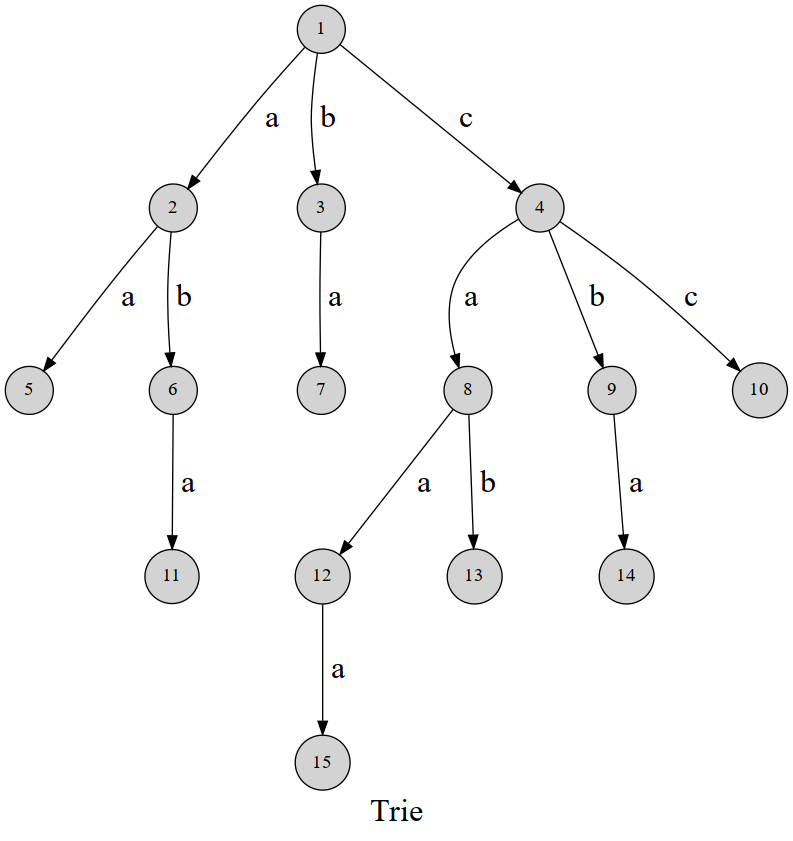
\includegraphics[height=5cm]{./images/trie1.png}
      \caption{字典树}
    \end{figure}
  \end{frame}

  \begin{frame}[fragile]{template}
    \begin{verbatim}
const int M = 1e6 + 10;
// son[i][c]表示第i个节点的第c个儿子 对应字符c的边
// cnt[i]表示以第i个节点结尾的字符串数量
int son[M][26], cnt[M], idx;
void insert(char str[]) { // 插入字符串
  int p = 0;
  for (int i = 0; str[i]; i++){
    int u = str[i] - 'a';
    // 不存在子节点就新建一个
    if (!son[p][u]) son[p][u] = ++ idx;
    p = son[p][u]; // 转移到子节点
  }
  cnt[p] ++; // 以该节点结尾的字符串数量+1
}\end{verbatim}
  \end{frame}

  \begin{frame}[fragile]{template}
    \begin{verbatim}
int query(char str[]) { // 查询字符串出现次数
  int p = 0;
  for (int i = 0; str[i]; i++) {
    int u = str[i] - 'a';
    if (!son[p][u]) return 0; // 不存在
    p = son[p][u]; // 转移到子节点
  }
  return cnt[p];
}\end{verbatim}
  \end{frame}

  \begin{frame}{检索字符串}
    给定一个字符集合,查询某个字符串是否在集合中出现过。\newline

    我们可以将字符串插入到字典树中,然后查询即可。
  \end{frame}

  \begin{frame}{最大异或值}
    给定一个长度为$n$的序列,求出序列中两个数的异或值最大的异或值。

    \begin{block}{思路}
      我们的想法是维护一个字典树,然后对于每一个数,我们求出这个数可以与字典树中的哪一个数异或得到最大值。最后在这些答案中选取最大值即可。
    \end{block}

    \begin{block}{查询最大异或值}
      \begin{itemize}
        \item 维护一颗二进制的字典树。
        \item 从高位到低位依次贪心地选择最大的数。
        \item 如果当前位为1,那么我们就尽量选择0,否则选择1。
        \item 如果当前位为0,那么我们就尽量选择1,否则选择0。
      \end{itemize}
    \end{block}
  \end{frame}

  \begin{frame} % 结束页
    \frametitle{End}
    \begin{center}
      \Huge{$THX\ 4\ Listening!$}
      \emph{:)}
    \end{center}
  \end{frame}
\end{document}